\documentclass[a4paper,num-refs]{oup-contemporary}

\journal{gigascience}

\usepackage{graphicx}
\usepackage{siunitx}
\usepackage{biblatex}
\addbibresource{references.bib}

%%% Flushend: You can add this package to automatically balance the final page, but if things go awry (e.g. section contents appearing out-of-order or entire blocks or paragraphs are coloured), remove it!
% \usepackage{flushend}

\title{Enter Title}

\author[1]{Enter Author}
\author[2]{Enter Author}
\author[3]{Enter Author}
\author[4]{Enter Author}
\author[5]{Enter Author}
\author[6]{Enter Author}

\affil[*]{\textbf{Target Price}: \textbf{Enter target price if possible} \\
\textbf{Investment Horizon}: Enter investment horizon}

\authnote{Birmingham Investment \&\ Finance Society, Asset Management Division}

\papercat{Company: enter company}

\runningauthor{enter a running page header}

\jvolume{1}
\jnumber{1}
\jyear{2025}

\begin{document}

\begin{frontmatter}

\maketitle

\begin{abstract}

Enter Introduction

\end{abstract}

\begin{keywords}

Enter keywords

\end{keywords}


\end{frontmatter}

%%%%%%%%%%%%%%%%%%%%%%%%%%%%%%%%%%%%%%%%%%%%%%%%%%%%%%%%%%%%%%%%%%%%%%%%%%%%%%%%%%%%%%%%%%%%%%%%%%%%%%%%%%%

\section{Front page top right corner it says stock outcome: ENTER}

To change this navigate to the oup-contemporary.cls file and use this search feature. Search for Stock outcome: BUY and then navigate to it using the up and down arrows then once found change it how you see fit

%%%%%%%%%%%%%%%%%%%%%%%%%%%%%%%%%%%%%%%%%%%%%%%%%%%%%%%%%%%%%%%%%%%%%%%%%%%%%%%%%%%%%%%%%%%%%%%%%%%%%%%%%%%

\section{If you need to input math equations, use chatgpt, there are many ways to do this, one note on this is if you have an equation inline with a paragraph (ie: not a block equation) use the dollar signs around the equation to get accurate compilation}

%%%%%%%%%%%%%%%%%%%%%%%%%%%%%%%%%%%%%%%%%%%%%%%%%%%%%%%%%%%%%%%%%%%%%%%%%%%%%%%%%%%%%%%%%%%%%%%%%%%%%%%%%%%

\section*{This style is for the main sections, start with the core proposition (ie: ur invesment thesis)}

\subsection{Use this for this style heading}

\subsubsection{Use this for this style heading}

\paragraph{Use this for this style heading}

\subparagraph{Use this for this style heading}

After each paragraph put 2 backslashes in the code after the last full stop to split things into paragraphs.

use the following code for bullet points
\begin{itemize}
    \item here is a bullet point
\end{itemize}

use the following code for numbered points
\begin{enumerate}
    \item here is a numbered point 
    \item and another
\end{enumerate}


%%%%%%%%%%%%%%%%%%%%%%%%%%%%%%%%%%%%%%%%%%%%%%%%%%%%%%%%%%%%%%%%%%%%%%%%%%%%%%%%%%%%%%%%%%%%%%%%%%%%%%%%%%%

\section{Images}

Below is an image. An important notice is that images either compile on the top of a collumn or on the bottom. Aim to use b! and t! in the first line to control where the image is compiled onto.\\

\begin{figure}[b!] %% preferably at bottom or top of column
\centering
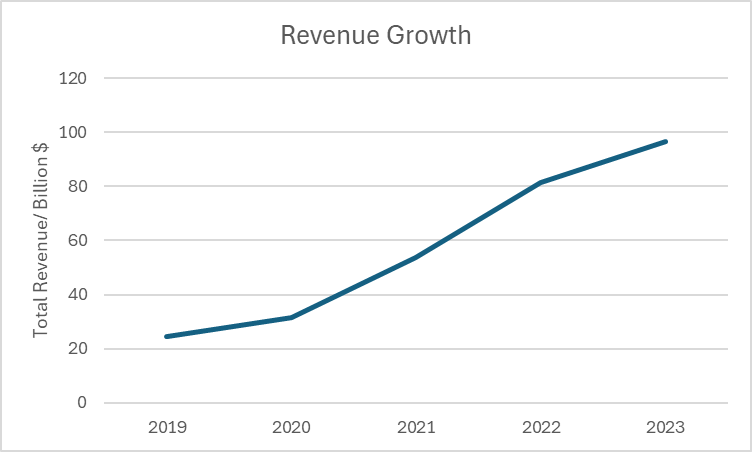
\includegraphics[width=\linewidth]{Images/RevenueGrowth.png}
\caption{Enter a suitable caption for the figure}\label{fig:example}
\end{figure}

The above code is how you input an image. To do this: simply upload the image using the button under the menu button where there is an upwards arrow with a line underneath. select your file, and drag and drop in the images folder to keep organised. Then you go to the line where it says includegraphics and change the Images/... to whatever image you want. I suggest to rename the image once uploaded to make it easier to track what you need to upload \\

Quick note, whenever you use the \&, \%, \$ symbol always put a backslash before it otherwise the pdf wont compile properly.\\

\section{Tables}

Below is an example of a table: 

\begin{table}[b!]
\caption{Historic Margin Ratios 2019-2023}\label{tab:example}
\setlength\tabcolsep{3pt} % Adjusts column spacing
\begin{tabular}{l r r r r r} % Defines number of columns & alignment
\toprule
Year & 2019 & 2020 & 2021 & 2022 & 2023 \\
\midrule
Gross Profit Margin & 16.6\% & 21.0\% & 25.3\% & 25.6\% & 18.25\% \\
Operating Margin & -0.28\% & 6.23\% & 12.12\% & 16.76\% & 9.19\% \\
Net Profit Margin & -3.51\% & 2.19\% & 10.26\% & 15.45\% & 15.50\% \\
\bottomrule
\end{tabular}
\end{table}

\subsection{How to Modify a Table in LaTeX}

If you are new to LaTeX, here’s a simple guide on how to modify a table step by step. If this is taking too long to understand, you can either just screenshot your excel tables and upload them as images, or you can manually input the data into chatgpt and use this table above and its code to prompt it "make me a table in this format" 

\subsubsection{Understanding the Table Structure}
The table consists of:
\begin{itemize}
    \item \textbf{\texttt{\textbackslash begin\{table\}[b!]}} – Starts the table and positions it (e.g., \texttt{[b!]} places it at the bottom of the page).
    \item \textbf{\texttt{\textbackslash caption\{...\}}} – Sets the title of the table.
    \item \textbf{\texttt{\textbackslash label\{...\}}} – Labels the table for referencing elsewhere.
    \item \textbf{\texttt{\textbackslash begin\{tabular\}\{l r r r r r\}}} – Defines the table format:
        \begin{itemize}
            \item \texttt{l} = Left-aligned text.
            \item \texttt{r} = Right-aligned numbers.
            \item The format \texttt{\{l r r r r r\}} means 1 left-aligned column (for "Year") and 5 right-aligned columns (for numeric data).
        \end{itemize}
    \item \textbf{\texttt{\textbackslash toprule}, \texttt{\textbackslash midrule}, \texttt{\textbackslash bottomrule}} – Draw horizontal lines.
\end{itemize}

\subsubsection{Updating Table Data}
To change values, simply update the numbers inside the table.  
For example, if you want to update the 2023 values, modify:

\begin{verbatim}
Gross Profit Margin & 16.6% & 21.0% & 25.3% & 25.6% & 20.0% \\  
Operating Margin & -0.28% & 6.23% & 12.12% & 16.76% & 11.5% \\  
Net Profit Margin & -3.51% & 2.19% & 10.26% & 15.45% & 16.2% \\  
\end{verbatim}

\subsubsection{Adding a New Column (e.g., 2024)}
To add a new year, update:\\

The column headers:\\
\begin{verbatim}
Year & 2019 & 2020 & 2021 & 2022 & 2023 & 2024 \\
\end{verbatim}
Each row (adding a value for 2024 at the end):\\
\begin{verbatim}



Gross Profit Margin & 16.6% & 21.0% & 25.3% & 25.6% & 18.25% & 19.5% \\
Operating Margin & -0.28% & 6.23% & 12.12% & 16.76% & 9.19% & 10.3% \\
Net Profit Margin & -3.51% & 2.19% & 10.26% & 15.45% & 15.50% & 16.1% \\

\end{verbatim}


Also update \texttt{\{l r r r r r\}} to \texttt{\{l r r r r r r\}} to match the new column.

\subsubsection{Adding a New Row}
If you need an extra financial metric, insert a new row inside the \texttt{tabular} block.  
For example, adding \textbf{EBITDA Margin}:

\begin{verbatim}
EBITDA Margin & 5.2% & 7.8% & 12.5% & 18.0% & 14.2% & 15.7% \\
\end{verbatim}

\subsubsection{Changing Formatting}
\textbf{(A) Align All Columns to the Left}  
Change:
\begin{verbatim}
\begin{tabular}{l r r r r r}
\end{verbatim}
to:
\begin{verbatim}
\begin{tabular}{l l l l l l}
\end{verbatim}

\textbf{(B) Increase Spacing Between Columns}  
Modify:
\begin{verbatim}
\setlength\tabcolsep{6pt}
\end{verbatim}
This increases the space between columns.

\textbf{(C) Change Column Widths}  
Use:
\begin{verbatim}
\begin{tabular}{p{3cm} p{2cm} p{2cm} p{2cm} p{2cm} p{2cm}}
\end{verbatim}
This sets the **first column** to **3cm wide** and number columns to **2cm wide**.

\subsection{Final Example (Updated Table)}

\begin{table}[b!]
\caption{Historic Margin Ratios 2019-2024}\label{tab:example}
\setlength\tabcolsep{6pt}  % Adjust spacing between columns
\begin{tabular}{l r r r r r r}  % Added new column for 2024
\toprule
Year & 2019 & 2020 & 2021 & 2022 & 2023 & 2024 \\
\midrule
Gross Profit Margin & 16.6\% & 21.0\% & 25.3\% & 25.6\% & 18.25\% & 19.5\% \\
Operating Margin & -0.28\% & 6.23\% & 12.12\% & 16.76\% & 9.19\% & 10.3\% \\
Net Profit Margin & -3.51\% & 2.19\% & 10.26\% & 15.45\% & 15.50\% & 16.1\% \\
EBITDA Margin & 5.2\% & 7.8\% & 12.5\% & 18.0\% & 14.2\% & 15.7\% \\
\bottomrule
\end{tabular}
\end{table}

\subsection{Summary}
\begin{itemize}
    \item \textbf{To update values} → Change the numbers in each row.
    \item \textbf{To add a new column} → Add data at the end of each row & update \texttt{\{l r r r r r\}}.
    \item \textbf{To add a new row} → Insert a new line inside \texttt{tabular}.
    \item \textbf{To adjust spacing} → Use \texttt{\textbackslash setlength\tabcolsep\{\}}.
    \item \textbf{To change column alignment} → Modify \texttt{\{l r r r r r\}} to \texttt{\{l l l l l l\}}.
\end{itemize}

Now you can modify LaTeX tables easily! 

%%%%%%%%%%%%%%%%%%%%%%%%%%%%%%%%%%%%%%%%%%%%%%%%%%%%%%%%%%%%%%%%%%%%%%%%%%%%%%%%%%%%%%%%%%%%%%%%%%%%%%%%%%%

\newpage


%%%%%%%%%%%%%%%%%%%%%%%%%%%%%%%%%%%%%%%%%%%%%%%%%%%%%%%%%%%%%%%%%%%%%%%%%%%%%%%%%%%%%%%%%%%%%%%%%%%%%%%%%%%

\section{References}

To modify the references, simply copy and paste your list of references into chatgpt and prompt it to convert the references into a .bib file format you can copy and paste into your overleaf envoirment. Access the references.bib file and copy and paste the output from chatgpt into this. all the other work is done for you. 

\section{Contributions}

Enter Contributions here

\newpage

\appendix

%%%%%%%%%%%%%%%%%%%%%%%%%%%%%%%%%%%%%%%%%%%%%%%%%%%%%%%%%%%%%%%%%%%%%%%%%%%%%%%%%%%%%%%%%%%%%%%%%%%%%%%%%%%

\newpage

\nocite{*}
\printbibliography





\end{document}
       